\section{Experiments and results}
\label{sec.results}

In this work the experiments used the OpenGL indirectly using the OpenSceneGraph~\cite{Burns2004}, a higher level, open-source, visualization framework. OpenSceneGraph provides a layer of abstraction over OpenGL in order to create the scene with memory managed objects, organized in a graph. This provides the dependencies of each object and optimises the memory utilization and rendering speed. Although the high-level of abstraction, it provides mechanisms to create custom operations if needed. The main advantage of using OpenSceneGraph for fishtank visualization is the easy abstraction with the windowing system, which is abstracted using object modeling strategy, and the multiple displays infrastructure. The visualization pipeline for the left and right screens introduces independent transformations for each screen defined by slave cameras. Each slave camera has view and projection transformations for each screen. In usual cases, those slave cameras are used to create a powerwall composed by many screens. The Figure~\ref{fig.osg_pipeline} show a schematic illustration of the pipeline for dual screens which are used to emulate an hologram, where the small arrows represent the slave cameras.

\begin{figure}[!hb]
\centering
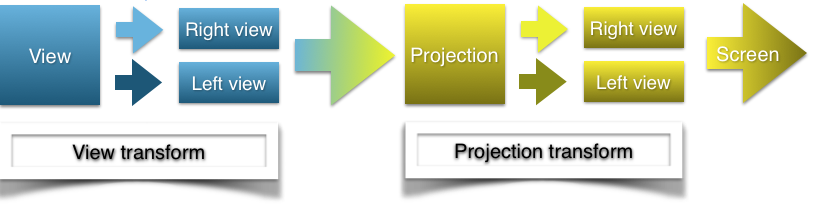
\includegraphics[width=\linewidth,keepaspectratio=true]{figs\osg_pipeline.png}
\caption{The viewing pipeline of OpenSceneGraph.}
\label{fig.osg_pipeline}
\end{figure}

In this investigation, a setup of two 3D displays forming a fish tank as in the illustration of Figure~\ref{fig.tv_setup}a. The fish tank has an extended field of view (FOV) of $120$ degrees between the displays, as illustrated in Figure~\ref{fig.tv_setup}b. They show the scene accordingly the view point of the viewer. The  position of the face of the viewer is tracked using a depth camera, in this case the Microsoft Kinect Sensor, and the viewer can use any of the stereo technologies presented in Section~ref{sec.stereo}. One drawback is the limitation of only one user but it can be overcome with a new display technology developed by Microsoft Research~\cite{Harris2010}. In order to create the space where the hologram is shown, the unconnected sides of the displays form the sides of a virtual 3D display where the origin of the hologram projected. The Figure~\ref{fig.tv_setup} show the setup of the experiment, with 2 stereo displays and the Kinect sensor. The area of tracking is shown by the frustum coming from the sensor. The original setup had 2 kinect sensors placed on the base of each display, but due hardware constrains, the setup has been reduced to only on sensor. The effect of this is a smaller tracking area, but it can be easily extended with extra hardware.

\begin{figure}[!ht]
\centering
\begin{tabular}{cc}
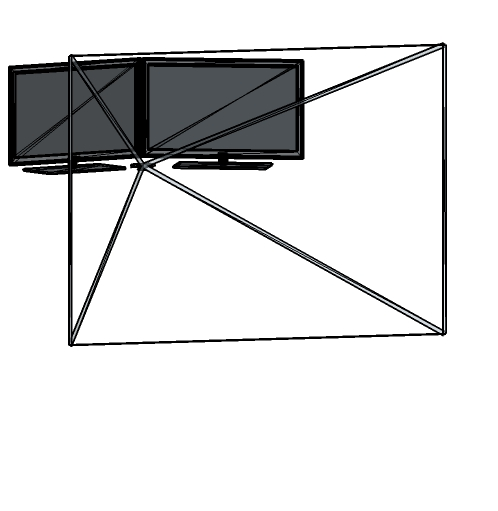
\includegraphics[width=0.45\linewidth,keepaspectratio=true]{figs\tv_setup_01.jpg}&
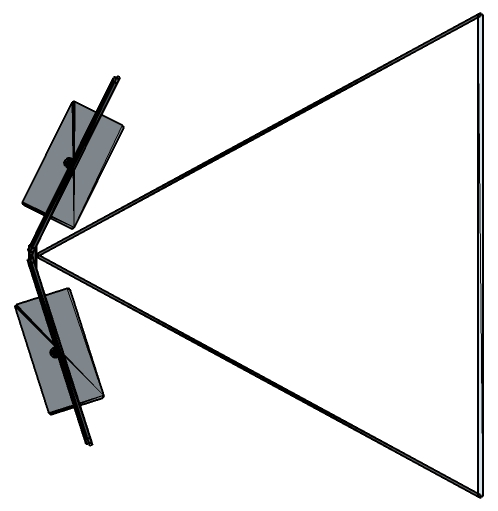
\includegraphics[width=0.45\linewidth,keepaspectratio=true]{figs\tv_setup_02.jpg}\\
(a) Stereo displays and Kinect & 
(b) Top view of fishtank
\end{tabular}
\label{fig.tv_setup}
\caption{Setup of the stereo displays and Kinect sensor}
\end{figure}

The implementation of the experiment used a face tracking library available in the Kinect SDK from Microsoft~\cite{Zhang2012}, which can track faces without prior training. The software can adjust the pitch angle of the sensor while it keeps the face in the center of the image. Ir order to remove the noise, the tracked movement is filtered by a step function in Equation{eq.step} ; that takes displacements $x$ greater than 1 cm or the average of the displacements $\mu_x$ if smaller. The Figure~\ref{fig.tracking} shows, on the right side, the video used in the face tracking and an overlay of a mask projected on of the video with the distance tracked. The attitude of the viewer, shown in the avatar on the left, is not used in this work because the hologram should stay on the same position for any rotation of the face.

\begin{equation}
  u(x)=\begin{cases}
    x, & \text{if $x>1$}.\\
    \mu_{x}, & \text{otherwise}.
  \end{cases}
  \label{eq.step}
\end{equation}

\begin{figure}[!ht]
\centering
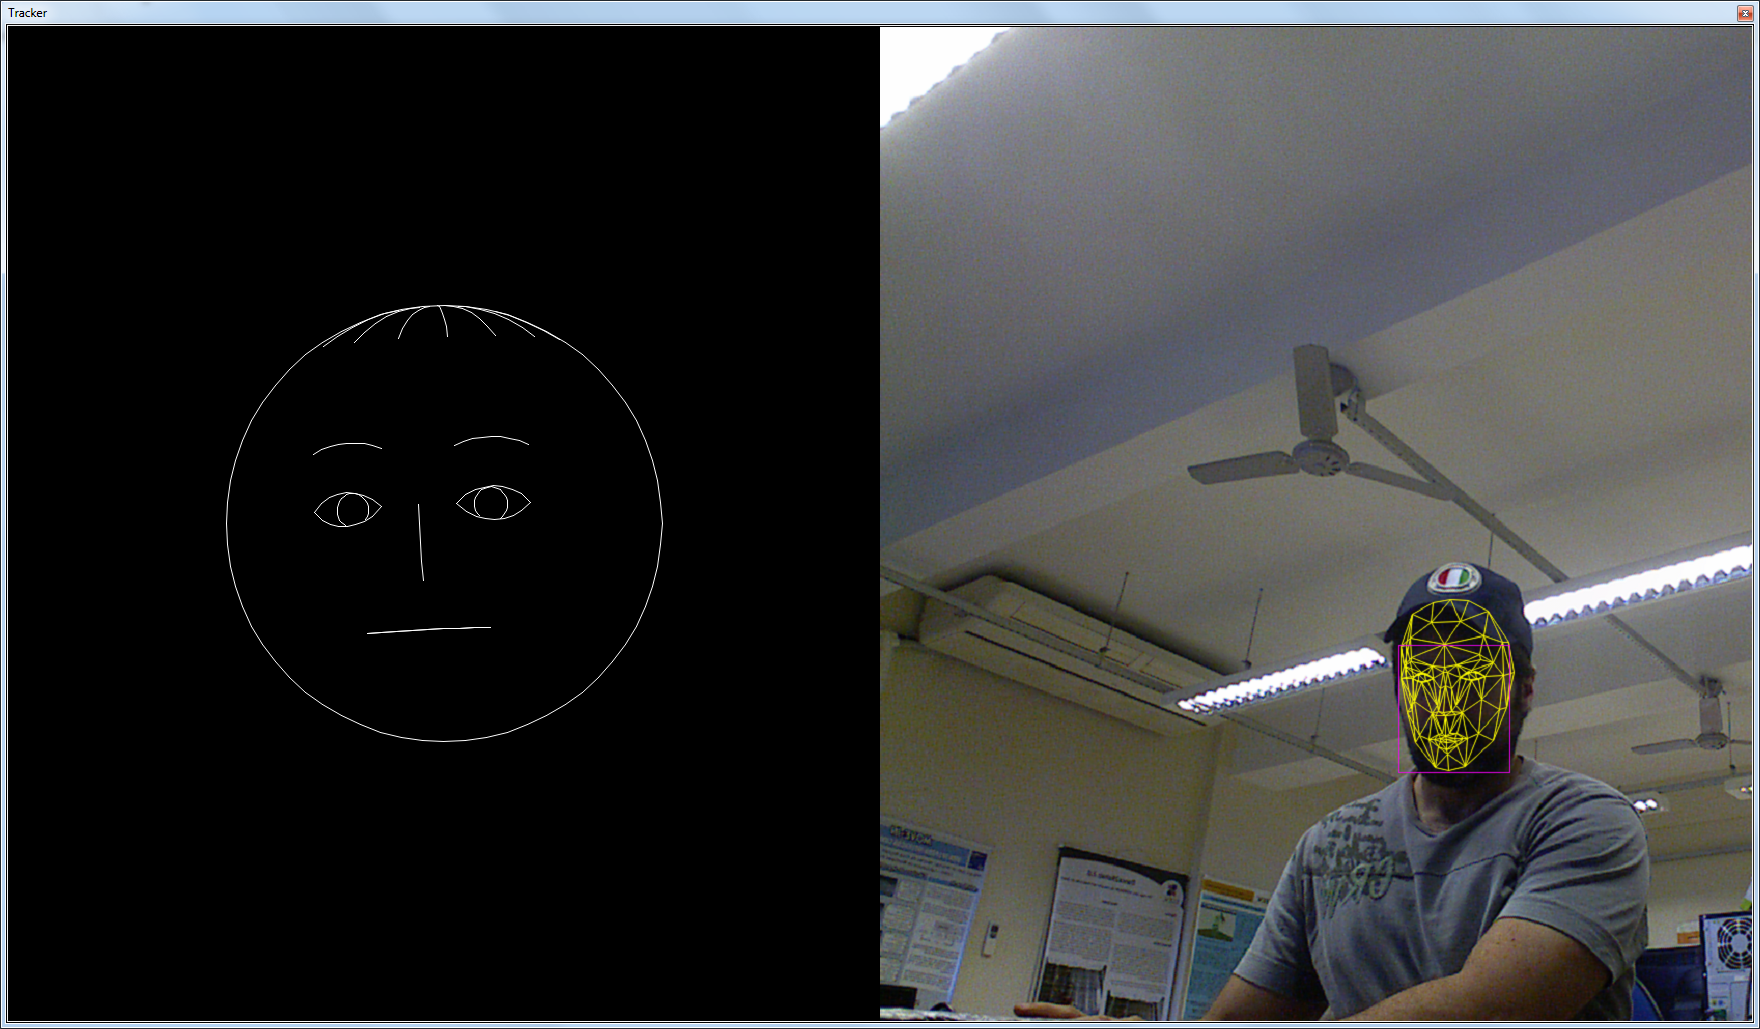
\includegraphics[width=0.9\linewidth,keepaspectratio=true]{figs\tracking.png}
\label{fig.tracking}
\caption{Face tracking module used to track the position of the viewer.}
\end{figure}

The stereo rendering uses the horizontal half of each screen for each eye as shown in Figure~\ref{fig.screens}. The projection is displaced by a horizontal offset on each slave view (small arrows) in projection transform of Figure~\ref{fig.osg_pipeline}. The width of bezel of the displays is taken in account in the offset to preserve an hidden continuity between the displays. The rotation of the screens is placed in slave cameras in the view transform.

\begin{figure}[!ht]
\centering
\begin{tabular}{cc}
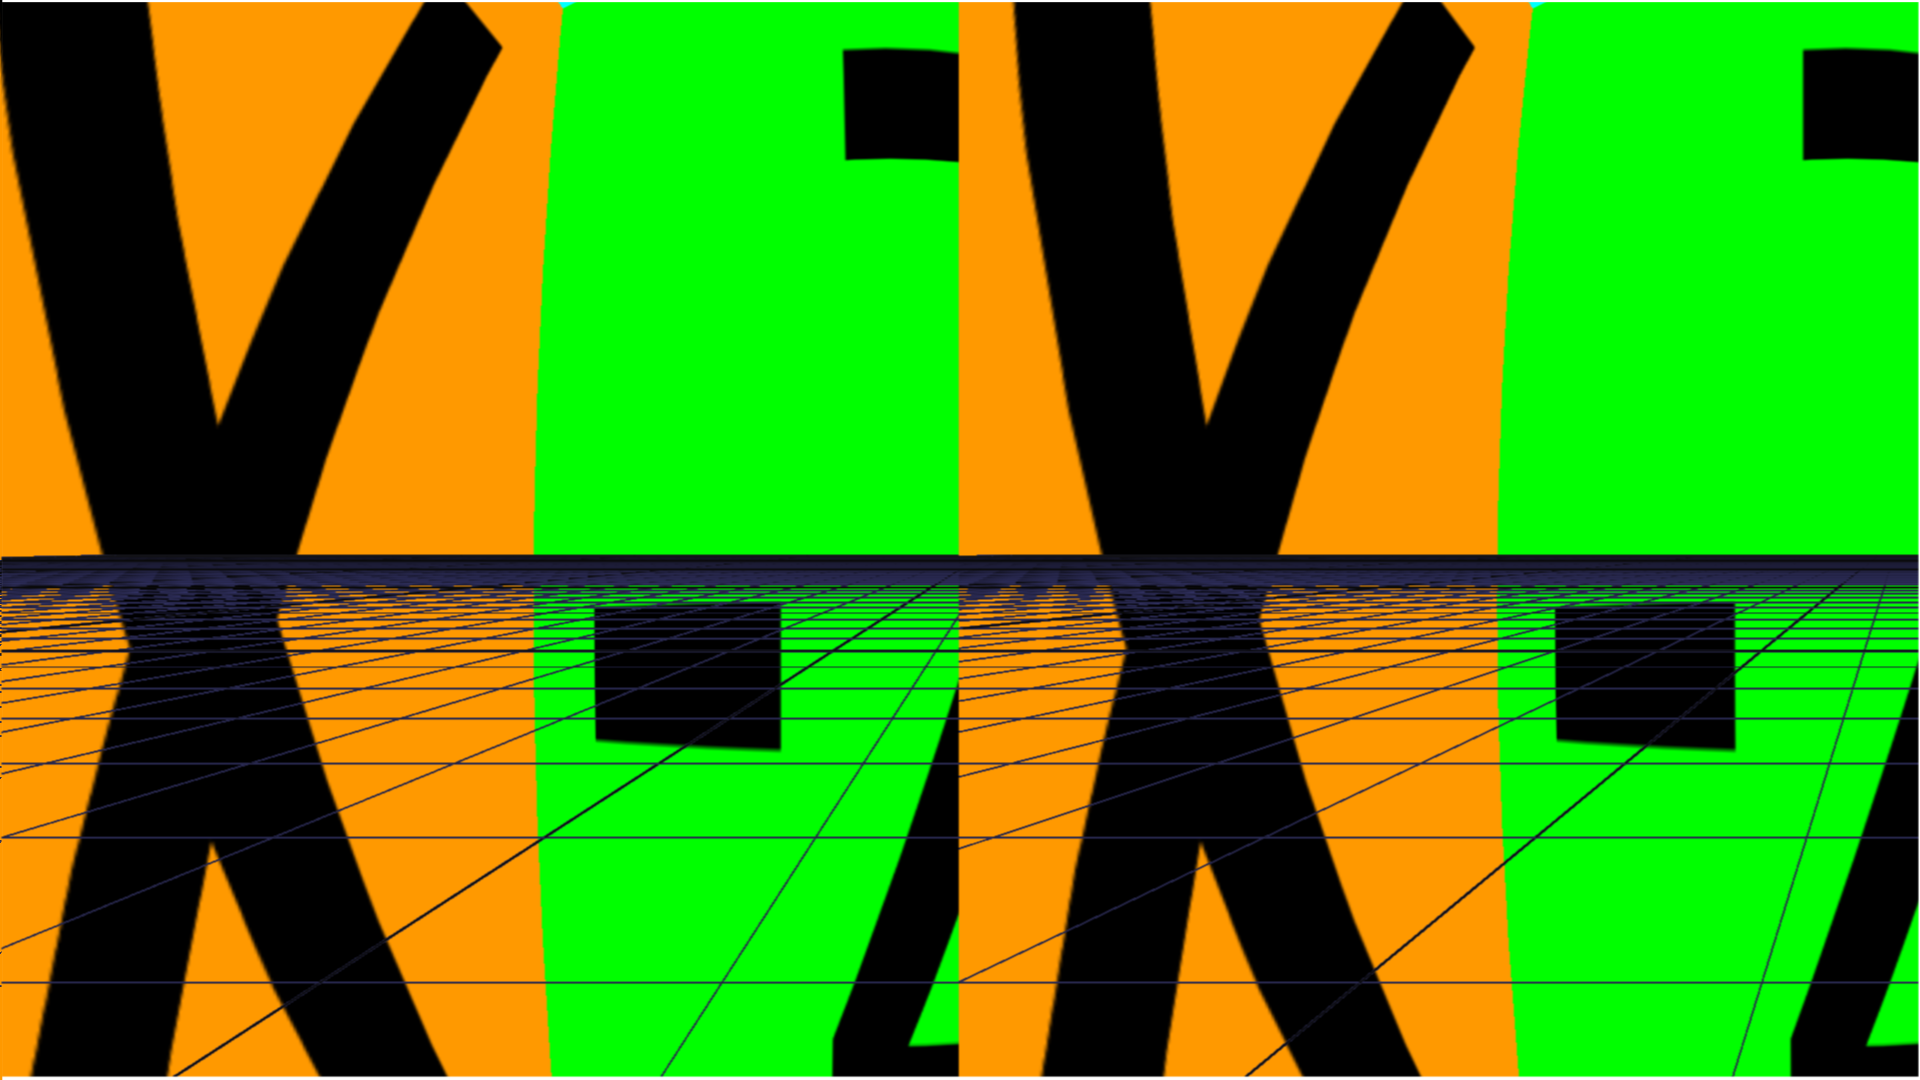
\includegraphics[width=0.45\linewidth,keepaspectratio=true]{figs\left_screen.png}&
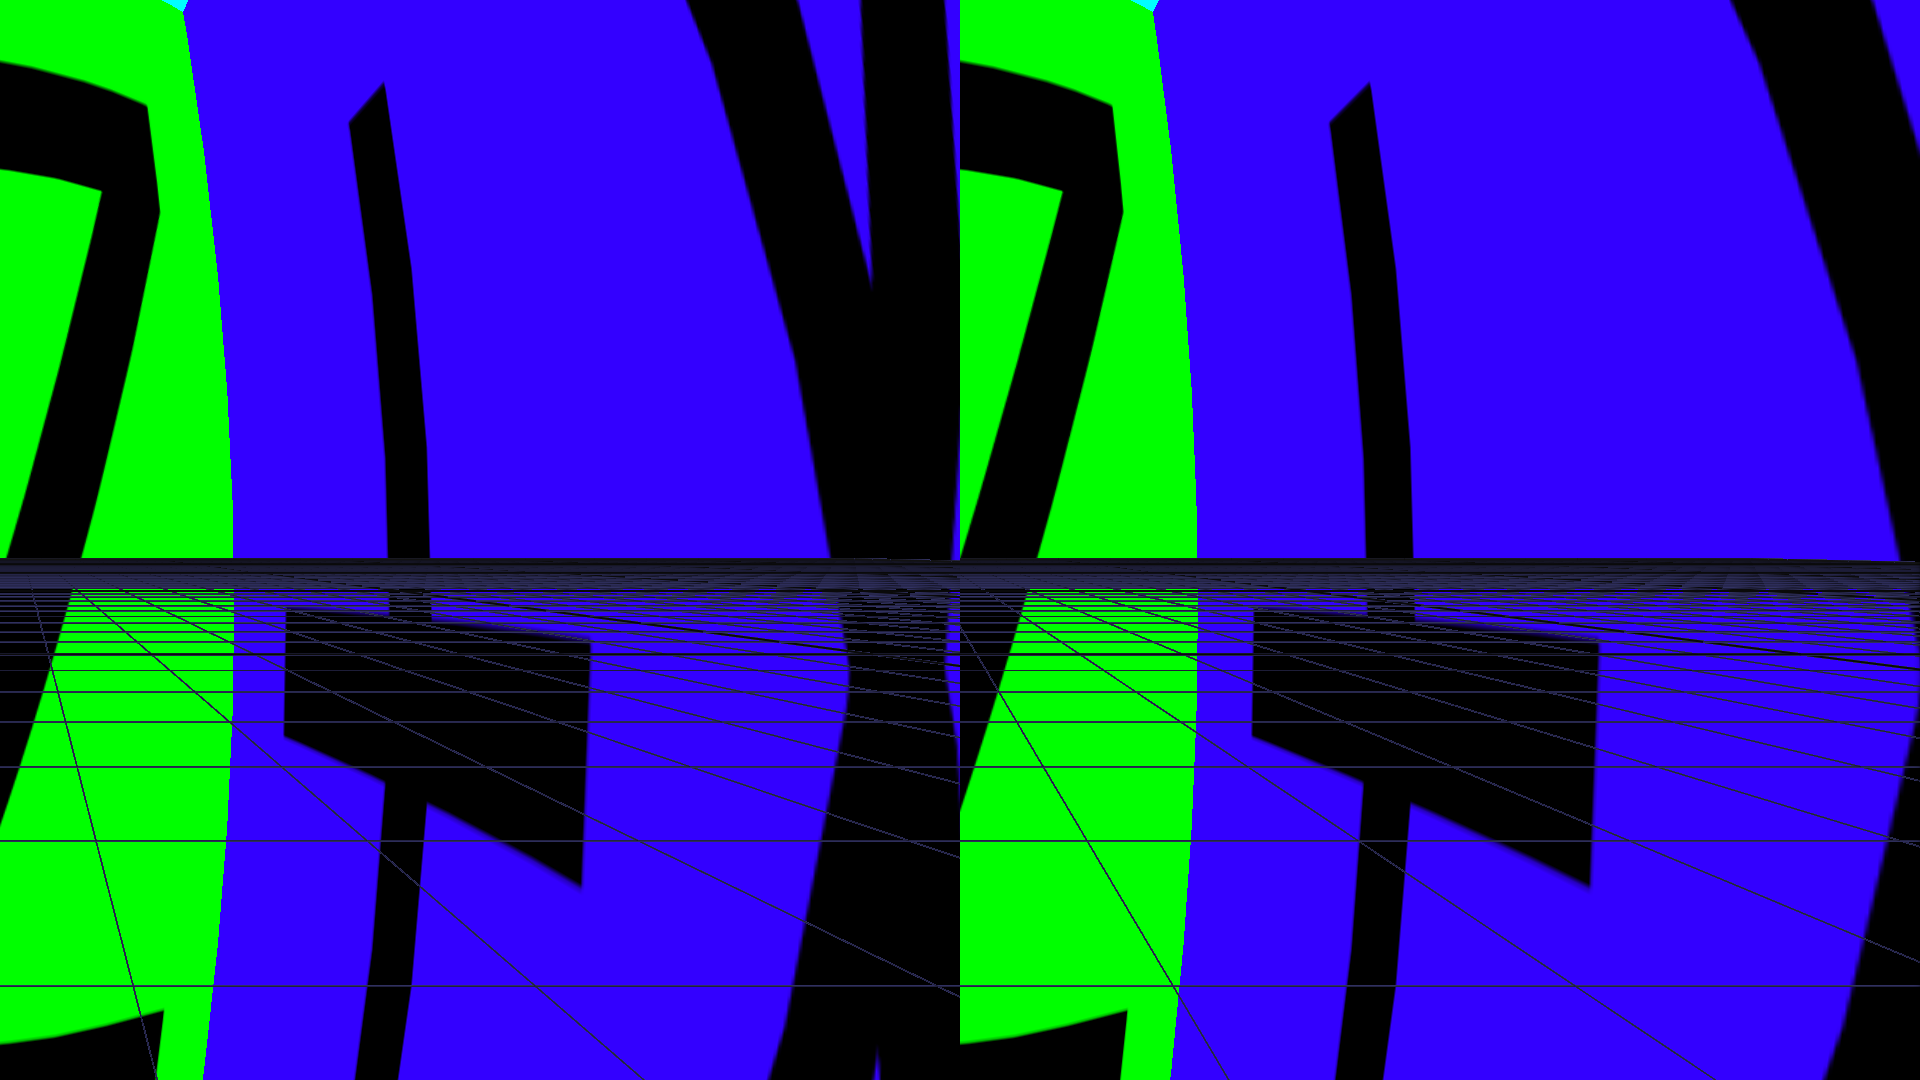
\includegraphics[width=0.45\linewidth,keepaspectratio=true]{figs\right_screen.png}\\
(a) Left display & 
(b) Right display
\end{tabular}
\label{fig.screens}
\caption{Vertical split of the stereo views.}
\end{figure}

The results of the experiments successfully emulated an hologram using the procedure described in Section~\ref{sec.hologram_emulation}, which changes the attitude of the models on the scene to produce the correct viewpoint. The experiments with the holographic projection transform are left for future work.





